\documentclass[nooutcomes]{ximera}
%% handout
%% space
%% newpage
%% numbers
%% nooutcomes


\newcommand{\RR}{\mathbb R}
\renewcommand{\d}{\,d}
\newcommand{\dd}[2][]{\frac{d #1}{d #2}}
\renewcommand{\l}{\ell}
\newcommand{\ddx}{\frac{d}{dx}}
\newcommand{\dfn}{\textbf}
\newcommand{\eval}[1]{\bigg[ #1 \bigg]}

\usepackage{multicol}

\renewenvironment{freeResponse}{
\ifhandout\setbox0\vbox\bgroup\else
\begin{trivlist}\item[\hskip \labelsep\bfseries Solution:\hspace{2ex}]
\fi}
{\ifhandout\egroup\else
\end{trivlist}
\fi} %% we can turn off input when making a master document
\usepackage{fullpage}
\title{Section 2.6: Continuity}  

\begin{document}
\begin{abstract}		\end{abstract}
\maketitle

%Problem1
\begin{problem}
	\begin{enumerate}
   	\item  Let $f(x) = \frac{x-1}{x^2 - 5x}$.  Then $f(2)=-\frac{1}{6}$ and $f(6)=\frac{5}{6}$, but there is no value of $c$ between $2$ and $6$ for which $f(c)=0$.  Does this fact violate the Intermediate Value Theorem?

      \begin{freeResponse}
        It does not violate the Intermediate Value Theorem.  $f$ is not continuous at 5 so the conditions of the IVT do not hold and therefore the IVT does not apply.
      \end{freeResponse}

	\item	True or False: At some time since you were born your weight in pounds exactly equaled your height in inches.
      \begin{freeResponse}
        True: if $w(t)$ represents your weight in pounds at time at time $t$ and $h(t)$ represents your height in inches at time $t$, then $w$ and $h$ are both continuous functions.  This implies $w - h$ is also continuous.
        If $t = 0$ is the moment you where born and $t = T_0$ is the present time, then $w(0) - h(0) < 0$ and $w(T_0) - h(T_0) > 0$.
        Hence by the Intermediate Value Theorem there is a point in the past, $t$, when $w(t)-h(t)=0$ and therefore your weight in pounds equaled your height in inches.
      \end{freeResponse}
	
	\end{enumerate}

\end{problem}

%problem 2
\begin{problem}
For the following function $g$ defined by
	
	$g(t) =   \left\{ \begin{array}{cl}
	5t + 7		 	&	\qquad \text{if } t < -3					\\ \\
	\frac{(t-1)(t+2)}{t+2}	&	\qquad \text{if } -3 \leq t < 1 \text{ and } t \neq -2	\\ \\
	4 \ln t				&	\qquad \text{if } t \geq 1					\end{array} \right.  $

  find the intervals where $g$ is continuous.  (\textbf{Important Note:} Write your answer as a list of intervals with each interval separated by a comma.)	

	\begin{freeResponse}
	The function $g$ is continuous on $(\infty, -3)$ since, in this interval, $g(t)=5t+7$ is a polynomial and therefore continuous on its domain.
  
  $g$ is not continuous at $t = -3$:
  \[
    \lim_{t \to -3^-} g(t) = \lim_{t \to -3^-} (5t+7) = 5(-3) + 7 = -8
  \]
  and
  \[
   \lim_{t \to -3^+} g(t)=g(-3) = \frac{(-3-1)(-3+2)}{-3+2} = \frac{4}{-1} = -4.
  \]

Although we have found $g$ is not continuous at $t = -3$, since $\lim_{t \to -3^+} g(t)=g(-3)$, $g$ is continuous from the right at $t=-3$.


  The function $g$ is continuous on $[-3, -2),(-2,1)$ since, in this interval, $g(t) = \frac{(t-1)(t+2)}{t+2}$ is a rational function whose denominator is not zero. $g$ is not continuous at $t=-2$ because it is not defined there.   $g$ is continuous on $(1, \infty)$, since, on this interval, $g(t) =  4 \ln(t)$ is a constant multiple of a  logarithmic function.

$g$ is continuous at $t = 1$:
  \[
    \lim_{t \to 1^-} g(x) = \lim_{t \to 1^-} \frac{(x-1)(x+2)}{x+2} = \frac{0}{3} = 0,
  \]
  and
\[ \lim_{t \to 1^+} g(x)=g(1) = 4 \ln(1) = 0\]


$g$ is continuous on the intervals \[(-\infty, -3), [-3, -2), (-2, \infty)\]
  \end{freeResponse}
	
		
	
\end{problem}
	
	
			

%problem 3			
\begin{problem}
Determine the value of a constant $b$ for which $f$ is continuous at $0$.
	
	$f(x) =   \left\{ \begin{array}{ll}
	\frac{2x+b}{x-5}	 	&	\qquad \text{if } x < 0	\\ \\
	\frac{x+16}{x^2-16}		&	\qquad \text{if } x \ge 0	\end{array} \right.  $

	\begin{freeResponse}
	
To have continuity at $x = 0$, the three conditions of continuity have to be satisfied.  These criteria are:
	\begin{center}
	  $f$ is defined at $x = 0$\\

     	 $\lim_{x \to 0} f(x)$ exists\\

    	  $\lim_{x \to 0} f(x) = f(0)$
	\end{center}

The first condition is satisfied.  In order to satisfy the second condition,  $\lim_{x \to 0} f(x)$ exists, we must verify that $\lim_{x \to 0} f(x)=\lim_{x \to 0^+} f(x)=\lim_{x \to 0^-} f(x)$.
That is, 
	\begin{align*}
	\lim_{x \to 0^+} f(x)&=\lim_{x \to 0^+} \left(\frac{x+16}{x^2-16}\right)=\frac{16}{-16}=-1\\
	\lim_{x \to 0^-} f(x)&=\lim_{x \to 0^-}\frac{2x+b}{x-5}=\frac{b}{-5}\\
	\implies & \lim_{x \to 0} f(x)=-1=\frac{-b}{5} \implies b=5
	\end{align*}

and $f(0)=-1$. Now we have found that  $\lim_{x \to 0} f(x)=f(0)=1$.
	
	\end{freeResponse}
\end{problem}
	
	


%problem 4	
\begin{problem}
  Use the Intermediate value theorem to find an interval in which you can guarantee that there is a solution to the equation $x^3 = x + \sin x + 1$.
  Do not use a graphing device or calculator to solve this problem!
  \begin{freeResponse}
    We have
    \begin{align*}
      x^3 = x + \sin x + 1 &\iff x^3 - x - \sin x - 1 = 0.
    \end{align*}
  Define $f(x) =  x^3 - x - \sin(x) - 1$.

    Since:\\
 $f(0) = (0)^3 - (0) - \sin(0)-1 = -1$ and \\
$f(\pi) = \pi^3 - \pi - \sin(\pi)-1 = \pi(\pi^2 - 1) - 1 > 3 \cdot (3^2 - 1) - 1 = 23$\\
We have: $-1<0<23$\\
and $f$ is continuous on $[0, \pi]$, the Intermediate Value Theorem implies there is some $c$ with $0 < c < \pi$ such that $f(c)=L= 0$, that is, $c^3 = c + \sin (c) + 1$.  So a possible interval is $[0,\pi]$.  Note: There are many possible solutions, e.g. $[1,4]$, etc.

	\begin{image}
	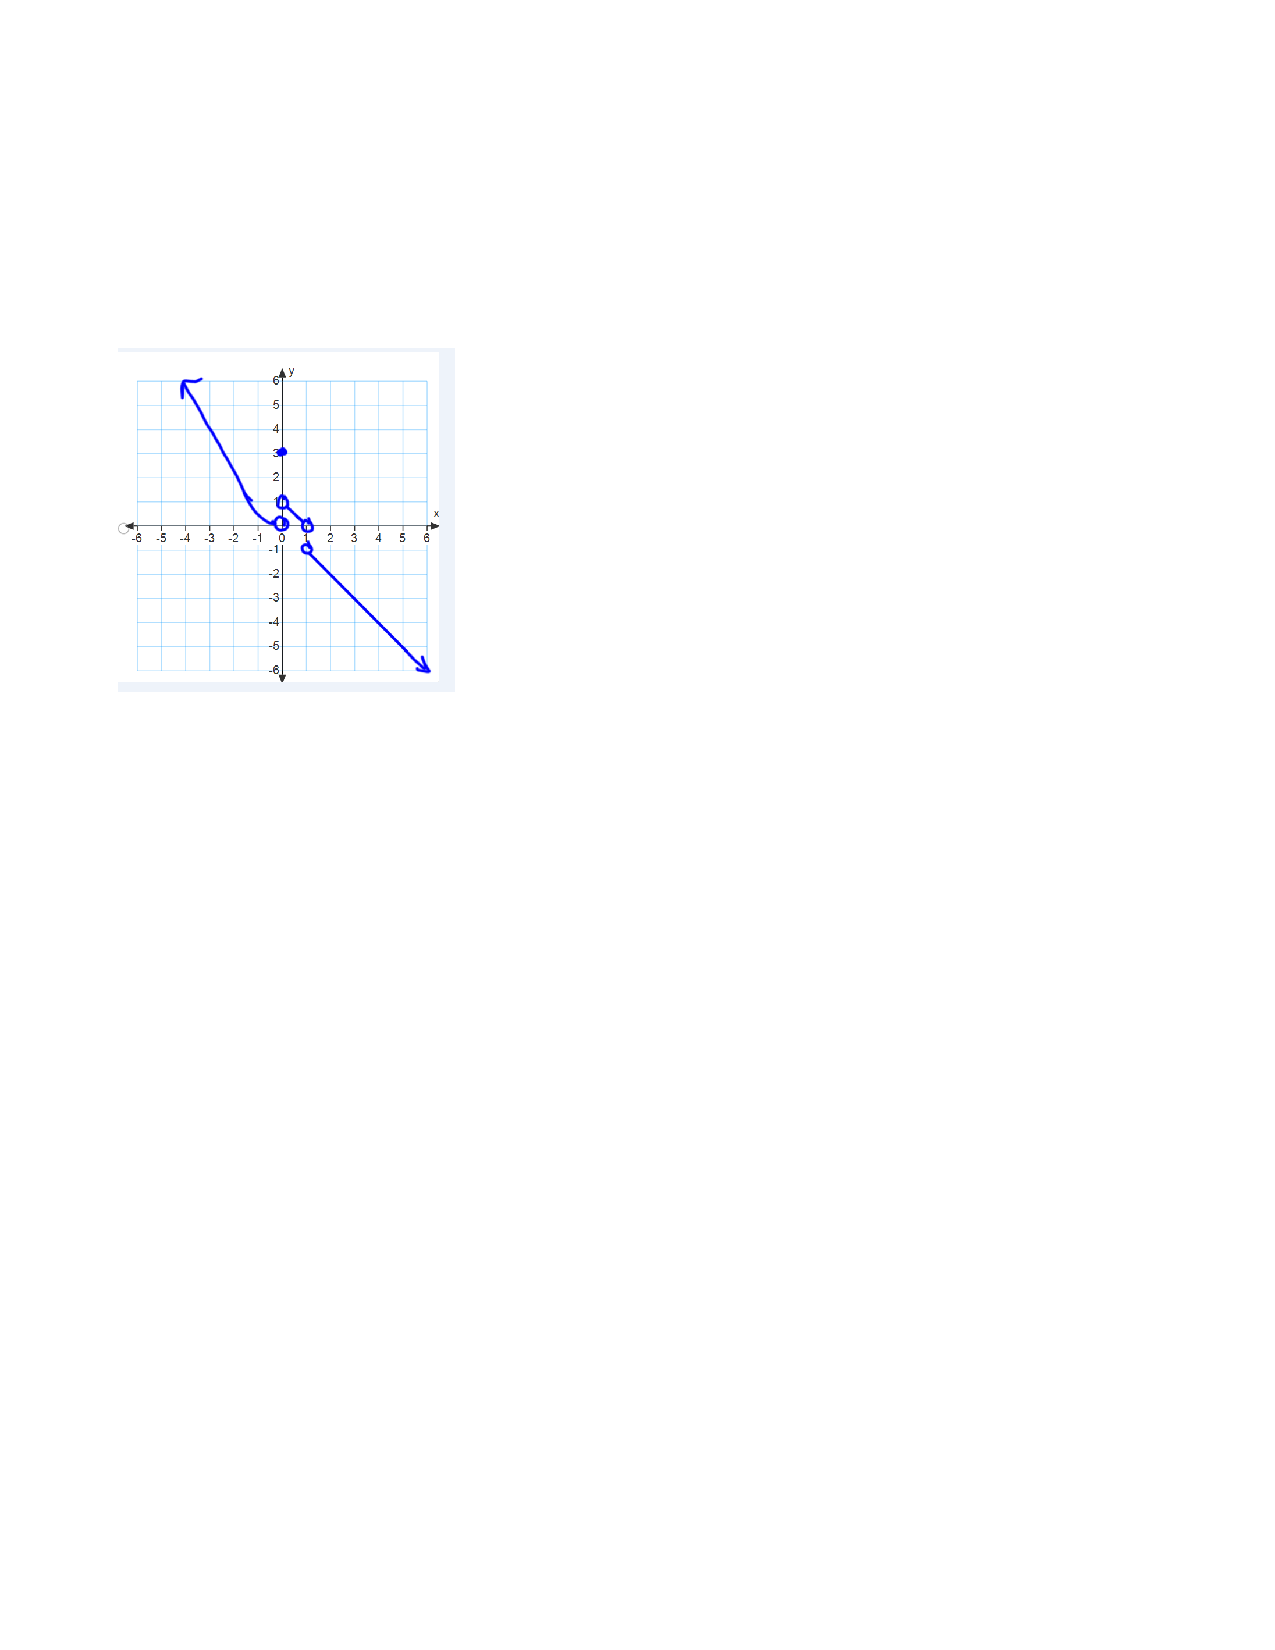
\includegraphics[scale=.5]{Figure3.png}
	\end{image}


  \end{freeResponse}
\end{problem}
	
%problem5
\begin{problem}
	\begin{enumerate}
	\item  True or False: If $f$ and $g$ are two functions defined on $(-1, 1)$, and if $\displaystyle \lim_{x \to 0} g(x) = 0$, then it must be true that $\displaystyle \lim_{x \to 0} (f(x) \cdot g(x)) = 0$.
  \begin{freeResponse}
    False: Suppose 
    \[
      f(x) =
      \begin{cases}
        \frac{1}{x} & \mbox{if $x \ne 0$}\\
        0 & \mbox{if $x = 0$}
      \end{cases}
    \]
    and $g(x) = x$.
    Then $\lim_{x \to 0} g(x) = 0$ but
    \[
      \lim_{x \to 0} (f(x) \cdot g(x)) = \lim_{x \to 0} \left( \frac{1}{x} \cdot x \right) = \lim_{x \to 0} 1 = 1.
    \]
  \end{freeResponse}

  \item True or False: If $f$ is continuous on $(-1, 1)$, and if $f(0) = 10$ and $\displaystyle \lim_{x \to 0} g(x) = 2$, then
  \[
    \lim_{x \to 0} \frac{f(x)}{g(x)} = 5.
  \]
  \begin{freeResponse}
    True: application of quotient rule.  Because $f$ is continuous, $lim_{x \to 0} f(x)=f(0)=10$
  \end{freeResponse}

	\item  True or False: If $f$ is continuous on $[1, 3]$, and if $f(1) = 0$ and $f(3) = 4$, then the equation $f(x) = \pi$ has a solution in $(1, 3)$.
  \begin{freeResponse}
    True: $f$ is continuous on $[1, 3]$, $f(1) = 0 < \pi < 4 = f(3)$, and the Intermediate Value Theorem implies there is some $x$ in $(1, 3)$ with $f(x) = \pi$.
  \end{freeResponse}

  \item True or False: Let $f$ be a positive function with vertical asymptote $x = 5$. Then
  \[
    \lim_{x \to 5} f(x) = \infty.
  \]
  \begin{freeResponse}
    False: Suppose $f$ is defined by
    \[
      f(x) =
      \begin{cases}
        \frac{1}{x - 5} & \mbox{if $x > 5$}\\
        2 & \mbox{if $x \le 5$}.
      \end{cases}
    \]
    
    Then $f$ has a vertical asymptote at $x = 5$:
    \begin{align*}
      \lim_{x \to 5^+} \underbrace{\frac{1}{x-5}} = \infty\ \text{because the limit is of the form:}\ \frac{\text{pos}}{0^+}
    \end{align*}

    But, $\displaystyle \lim_{x \to 5^-} f(x) = 2$.\\
	Therefore, $lim_{x \to 5} f(x)$ does not exist

  \end{freeResponse}
\end{enumerate}
\end{problem}

%problem 6
\begin{problem}
Let 
    \[
      h(u) =
      \begin{cases}
        \frac{u^2-5u+4}{u - 4} & \mbox{if $u < 4$}\\ \\
         \frac{-\sqrt{u+4}}{u - 6} & \mbox{if $u \ge 4, u \ne 6$}.
      \end{cases}
    \]

\begin{enumerate}
	\item What is the domain of $h$?

	\begin{freeResponse}
	For values of $u<4$ we check $\frac{u^2-5u+4}{u - 4}$.  This piece of the function is defined everywhere on $(-\infty,4)$\\
	For values of $u\geq 4$ we check $\frac{-\sqrt{u+4}}{u - 6}$. This piece of the function is defined everwhere except $u=6$.  So $h$ is defined on $[4,6)\cup(6,\infty)$
	The domain is $(-\infty,6)\cup(6,\infty)$
	\end{freeResponse}

	%x
	\item Find all vertical asymptotes of $h$ and justify using limits.

	\begin{freeResponse}
	The only candidates are $u=6$ and $u=4$.
	
	\begin{align*}
	&\lim_{u \to 6^+}\frac{-\sqrt{u+4}}{u - 6}=-\infty\ \text{because it is of the form:}\ \frac{\text{neg}}{0^+}\\ \\
	&\lim_{u \to 4^-} \frac{u^2-5u+4}{u - 4}=\lim_{u \to 4^-} \frac{(u-1)(u-4)}{u - 4}=\lim_{u \to 4^-} (u-1)=3 \\ \\
	&\lim_{u \to 4^+} \frac{-\sqrt{u+4}}{u - 6}=\frac{-\sqrt{8}}{-2}=\sqrt{2}
	\end{align*}
	The only vertical asympote is $u=6$
	\end{freeResponse}
	
	\item Find all horizontal asymptotes of $h$ and justify using limits.
	\begin{freeResponse}
	\begin{align*}
	\lim_{u \to \infty}\frac{-\sqrt{u+4}}{u - 6}&=\lim_{u \to \infty}\frac{-\frac{\sqrt{u+4}}{\sqrt{u}}}{\frac{u - 6}{\sqrt{u}}}\\ \\
	&=\lim_{u \to \infty}\frac{-\sqrt{\frac{u+4}{u}}}{\frac{u}{\sqrt{u}} - \frac{6}{\sqrt{u}}}\\ \\
	&=\lim_{u \to \infty}\frac{\sqrt{1+\frac{4}{u}}}{\sqrt{u} - \frac{6}{\sqrt{u}}}\\ \\
	&=0\\ \text{because it is of the form:}\ \frac{\text{pos}}{\infty}
	\end{align*}
	This indicates that $y=0$ is a horizontal asymptote.\\
	Checking as $x$ approaches $-\infty$ we have:
	\begin{align*}
	\lim_{u \to -\infty}\frac{u^2-5u+4}{u - 4}=\lim_{u \to -\infty} \frac{(u-1)(u-4)}{u - 4}=\lim_{u \to -\infty} (u-1)= -\infty
	\end{align*}
 Therefore, there is no horizontal asymptote as $x$ approaches $-\infty$
	
	\end{freeResponse}

	%d
	\item Where is $h$ continuous?

	\begin{freeResponse}
		For values of $u<4$ we check $\frac{u^2-5u+4}{u - 4}$.  This piece of the function is continuous everywhere on $(-\infty,4)$ \\
	For values of $u>4$ we check $\frac{-\sqrt{u+4}}{u - 6}$. This piece of the function is continuous everwhere where defined: $(4,6),(6,\infty)$\\

	We need to check $u=4$ for continuity. A function is continuous at a point $a$ if:
	\begin{center}
	  $f$ is defined at $x = a$\\

     	 $\lim_{x \to a} f(x)$ exists\\

    	  $\lim_{x \to a} f(x) = f(a)$
	\end{center}

$h$ is defined at $u=4$, $h(4)=\frac{-\sqrt{4+4}}{4 - 6}=\sqrt{2}$\\
Next we check if  $\lim_{u \to 4} h(u)$ exists.  That is, does $\lim_{u \to 4^-} h(u)=\lim_{u \to 4^+} h(u)$ ?

	\begin{align*}
	\lim_{u \to 4^-} h(u)&=\lim_{u \to 4^-}\frac{u^2-5u+4}{u - 4}\\
	& \text{This is of the form:}\ \frac{0}{0^-}\ \text{so we need to do more algebra}\\
	&=\lim_{u \to 4^-}\frac{(u-4)(u-1)}{(u-4)}\\
	&=\lim_{u \to 4^-}(u-1)\\
	&=4-1\\
	&=3 \\ \\
	\lim_{u \to 4^+} h(u)&=\lim_{u \to 4^+}\frac{-\sqrt{u+4}}{u - 6}\\
	&=\frac{-\sqrt{4+4}}{4 - 6}\\
	&=\frac{-\sqrt{8}}{-2}\\
	&=\sqrt{2}\\ \\
	&\lim_{u \to 4^-} h(u)\ne \lim_{u \to 4^+} h(u) \implies \lim_{u \to 4} h(u)\ \text{does not exist}
	\end{align*}
Thus $h(u)$ is not continuous at $u=4$. Remark: Since $\lim_{u \to 4^+} h(u)=h(4)$, $h$ is right continuous at $u=4$.   Its intervals of continuity are $(-\infty,4),[4,6),(6,\infty)$

	\end{freeResponse}



\end{enumerate}
\end{problem}
								
%problem7
\begin{problem}				
	Use the graph of $f$ to answer the questions below.
	\begin{image}
	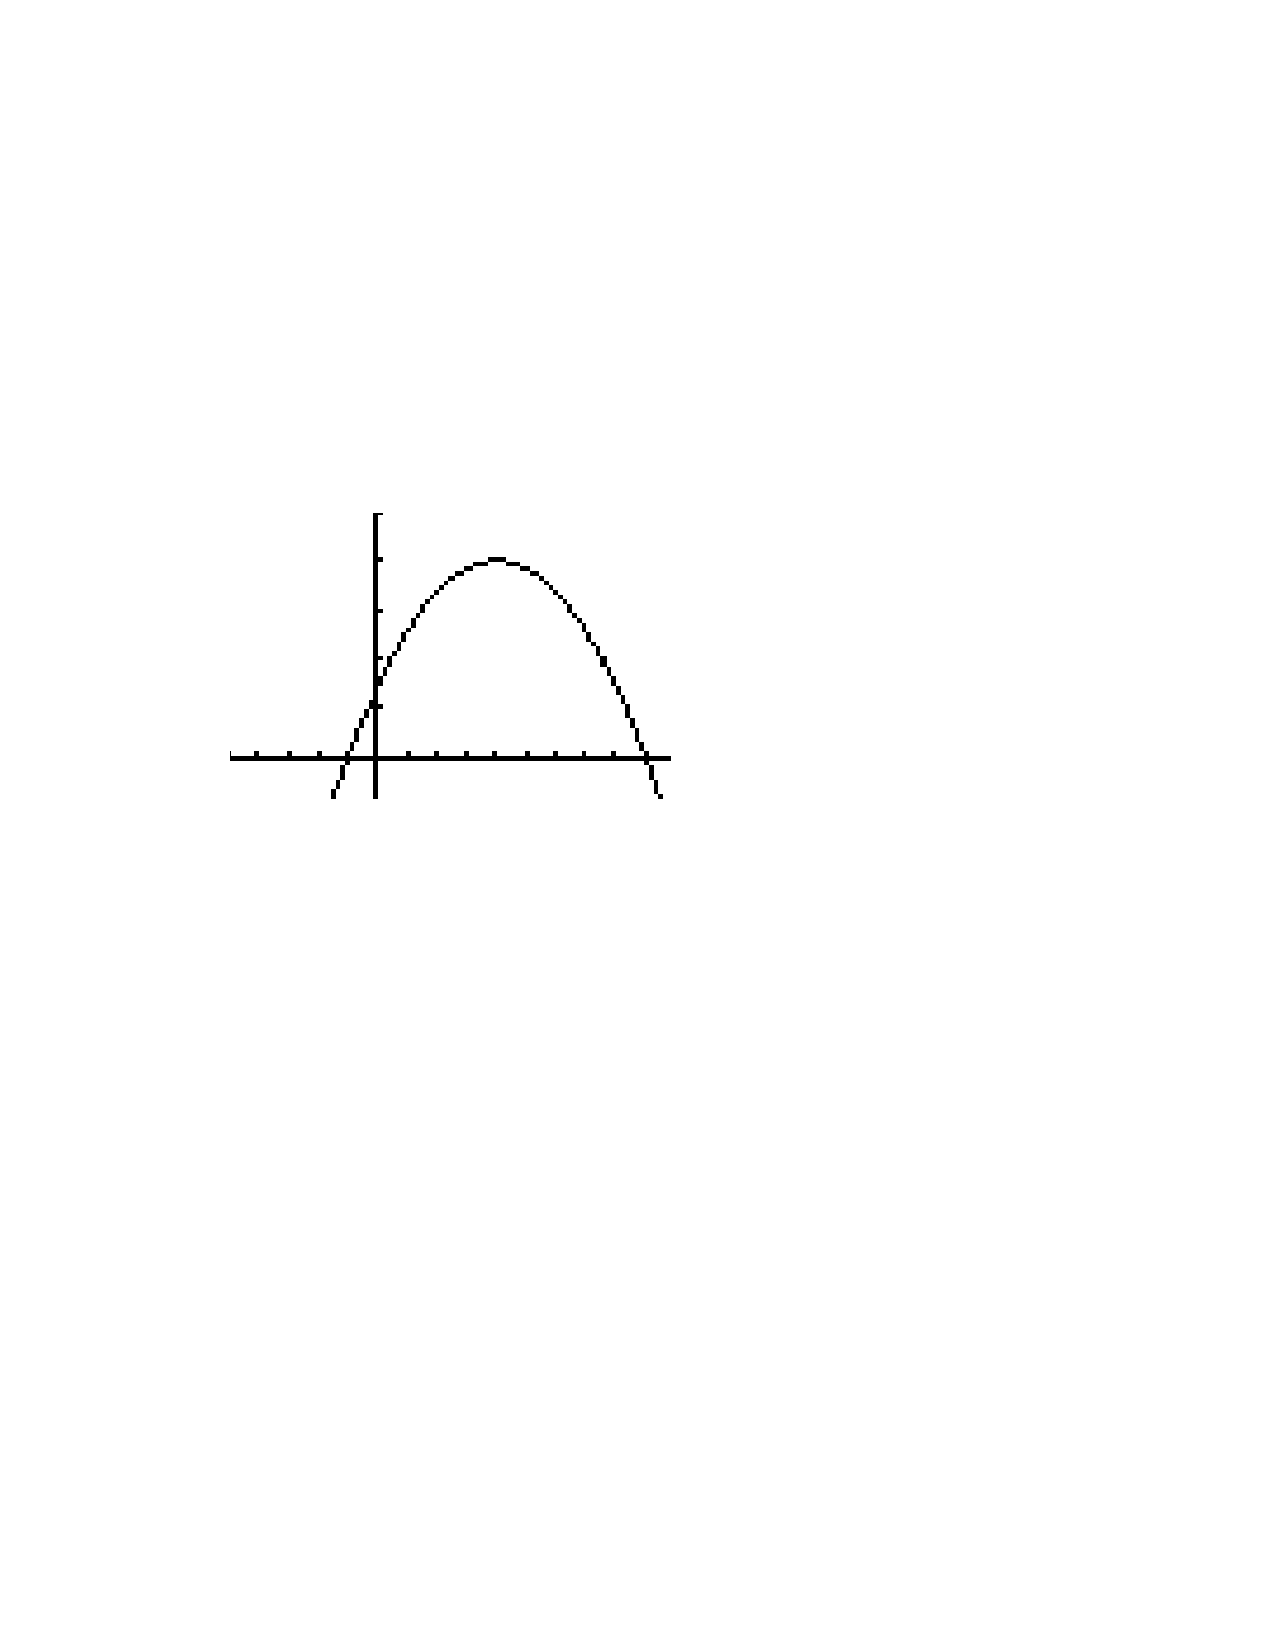
\includegraphics[scale=.5]{Figure1.png}
	\end{image}

	\begin{enumerate}		
		\item State the domain of $f$.
		
		\begin{freeResponse}
			$(-\infty,-1)\cup(-1,\infty)$
		\end{freeResponse}

		\item Find the following values or state "does not exist":
			\begin{enumerate}
 			\item $\lim_{x \to 2^-} f(x)=$
			\item $\lim_{x \to 2^+} f(x)=$
			\item $\lim_{x \to 2} f(x)=$
			\item $\lim_{x \to -1} f(x)=$
			\item $\lim_{x \to 3} f(x)=$
			\item $\lim_{x \to -\infty} f(x)=$
			\item $f(-1)=$
			\end{enumerate}
		\begin{freeResponse}
			\begin{enumerate}
 			\item $\lim_{x \to 2^-} f(x)=\infty$
			\item $\lim_{x \to 2^+} f(x)=-3$
			\item $\lim_{x \to 2} f(x)\ \text{Does not exist}$
			\item $\lim_{x \to -1} f(x)=1$
			\item $\lim_{x \to 3} f(x)=-4$
			\item $\lim_{x \to -\infty} f(x)=1$
			\item $f(-1)\  \text{Does not exist}$
			\end{enumerate}
		\end{freeResponse}


		\item State the equation of any vertical asmyptotes.
			\begin{freeResponse}
			$x=2$
			\end{freeResponse}


		\item State the equation of any horizontal asymptotes.
			\begin{freeResponse}
			$y=1$
			\end{freeResponse}
	
		\item Find the intervals of continuity.
			\begin{freeResponse}
			$(-\infty,-1),(-1,2),[2,\infty)$
			\end{freeResponse}
	
	\end{enumerate}
\end{problem}


%problem8
\begin{problem}
Suppose a taxi ride costs $\$7.50$ for the first mile (or any part of the first mile), plus an additional $\$1.00$ for each additional mile (or any part of a mile).
\begin{enumerate}
	\item Graph the function $c=f(t)$ that gives the cost of a taxi ride for $t$ minutes, for $0 \le t \le 5$.
		\begin{freeResponse} \hfil
	\begin{image}
	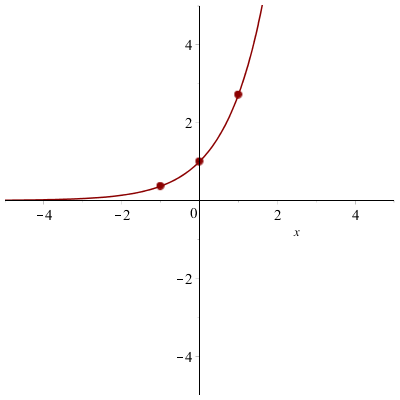
\includegraphics[scale=.5]{Figure5.png}
	\end{image}
		\end{freeResponse}

	\item Evaluate $\lim_{t \to 2.9}f(t)$
		\begin{freeResponse}
$\lim_{t \to 2.9}f(t)=9.5$
		\end{freeResponse}
	\item Evaluate $\lim_{t \to 3^-}f(t)$ and $\lim_{t \to 3^+}f(t)$		
		\begin{freeResponse}
$\lim_{t \to 3^-}f(t)=9.5$ and $\lim_{t \to 3^+}f(t)=10.5$	
		\end{freeResponse}
	\item Interpret the meaning of the limits in part (c).
		\begin{freeResponse}
As the number of miles the taxi drives approaches 3, the cost of the taxi ride is \$9.50.  If one drives for a bit more than 3 miles, the cost is \$10.50.
		\end{freeResponse}
	\item On what interals is the function $c$ continuous?  Explain.
		\begin{freeResponse}
			$(0,1],(1,2],(2,3],(3,4],(4,5]$
		\end{freeResponse}
\end{enumerate}
\end{problem}

%problem9
\begin{problem} \hfil
\begin{enumerate}

\item Given function $f$ on an interval $[a,b]$:

\begin{enumerate}
\item What are the conditions of the Intermediate Value Theorem?

	\begin{freeResponse}
$f$ is continuous on the interval $[a,b]$ 
	\end{freeResponse}
\item What is the conclusion of the Intermediate Value Theorem?
	\begin{freeResponse}
For any number $L$ strictly between $f(a)$ and $f(b)$, there is at least one number $c$ in $(a,b)$ satisfying $f(c)=L$.  This means that for any $L$ strictly between $f(a)$ and $f(b)$, the horizontal line $y=L$ intersects the graph of $f$. \\\\
	\end{freeResponse}

\end{enumerate}
	\item Given the four functions on the interval $[1,6]$, answer the questions below. 
	
	\begin{image}
	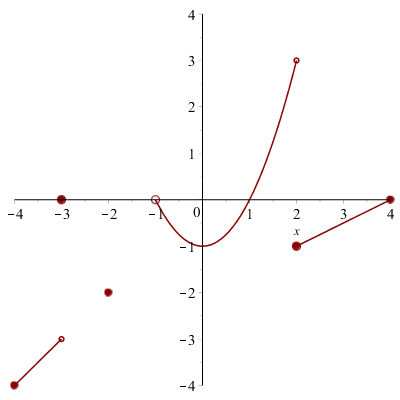
\includegraphics{Figure2.png}
	\end{image}

\begin{enumerate}
	\item For each of the functions I through IV, indicate $f(1)$ and $f(6)$.  Then mark the interval of all numbers strictly between $f(1)$ and $f(6)$, on the y-axis.
	\begin{freeResponse} \hfil
	\begin{image}
	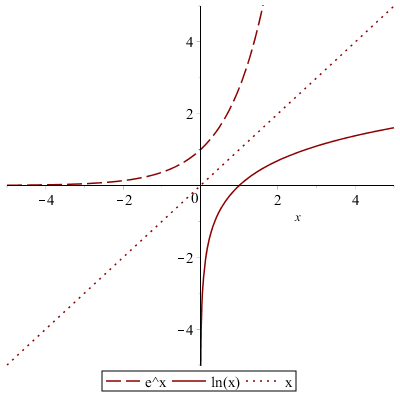
\includegraphics[scale=.6]{Figure4.png}
	\end{image}
	\end{freeResponse}

	\item For each of the functions I through IV, write an interval of all numbers strictly between $f(1)$ and $f(6)$
		\begin{freeResponse}
		$f=I$: $(3,4)$\\
		$f=II$: $(2,3)$\\
		$f=III$: $(1,5)$\\
		$f=IV$: $(1,5)$
		\end{freeResponse}
	\item List the functions that satisfy the conditions of the Intermediate Value Theorem on $[1,6]$
		\begin{freeResponse}
		Only function IV is continuous on $[1,6]$
		\end{freeResponse}
	\item For which of the functions is the following statement true: For any number $L$ strictly between $f(1)$ and $f(6)$, there exists a number $c$ in $(1,6)$ satisfying $f(c)=L$.
		\begin{freeResponse}
		The statement is true for functions I and IV
		\end{freeResponse}

	\item Does the function III satisfy the conclusion of the Intermediate Value Theorem?  Why or why not?
	\begin{freeResponse}
	No, function $f= III$ does not satisfy the conclusion of the IVT.  For example, take $L=1.5$.  $f(c)=1.5$ has no solution in $(1,6)$.  Draw the horizontal line $y=1.5$.  What do you notice?  This line does not intersect the graph of function III.  What does this mean?  The function does not attain that value, $1.5$.  So there is no $c$ in $(1,6)$ such that $f(c)=1.5$.
	\end{freeResponse}


	\end{enumerate}
\end{enumerate}

\end{problem}
\end{document} 
















